\subsection{Funciones de C++}

\begin{frame}[plain]
  \centering
  \color{theme-brand-color}
  \Huge \textbf{Funciones de C++}
\end{frame}

\begin{frame}{Lower y Upper Bound}
  \begin{figure}[H]
    \centering
    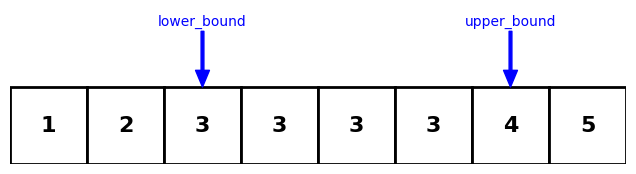
\includegraphics[width=0.85\textwidth]{./assets/lower_upper.png}
  \end{figure}
  \begin{itemize}
  \item \texttt{lower\_bound}: Apunta al primer elemento mayor o igual a 3.
  \item \texttt{upper\_bound}: Apunta al primer elemento mayor a 3.
  \end{itemize}
\end{frame}

\begin{frame}[fragile]{Implementación}
\begin{columns}[T] 
\column{0.5\textwidth}
\inputminted[
    fontsize=\small,
    linenos
]{cpp}{code/lower_bound.cpp}
\column{0.5\textwidth}
\inputminted[
    fontsize=\small,
    linenos
]{cpp}{code/upper_bound.cpp}
\end{columns}
\end{frame}


\begin{frame}{STL}
  \begin{itemize}
  \item \texttt{bool binary\_search(first, last, val, comp)}
  \item \texttt{iterator lower\_bound(first, last, val, comp)}
    \begin{itemize}
    \item Si todos son mayores regresa \texttt{end()}.
    \item Índice en arreglo
      
      \texttt{int k = lower\_bound(a, a+n, x) - a}
    \end{itemize}
  \item \texttt{iterator upper\_bound(first, last, val, comp)}
    \begin{itemize}
    \item Si todos son menores o iguales regresa \texttt{end()}
    \item Cantidad de ocurrencias
      
      \texttt{int count = upper\_bound(v.begin(), v.end(), x) -
        lower\_bound(v.begin(), v.end(), x)}
    \end{itemize}
  \item \texttt{pair<iterator, iterator> equal\_range(first, last, val, comp)}
    \begin{itemize}
    \item Elementos del iterador

      \texttt{*er.first, *er.second}.
    \end{itemize}
  \end{itemize}
\end{frame}
